\documentclass[../../main.tex]{subfiles}
\graphicspath{{\subfix{../../res/}}}
\begin{document}

There is many ways of defining what is student success. From a societal or governmental (administrative) point of view, the definition can vary technically, but tell the same thing nonetheless. For institution, student's success can be define as the percentage of student who got their diploma, in how many years and the overall grade score. For governments and administration, it could be define as the success rate (number of graduation and overall grades) of national exam. As for the student point of view, success is getting their diploma by the end of the usual cursus. Some may evaluate their success on the grades they've got as well, which can be a factor to determine students who are motivated not only by just getting their diploma but also in actually succeeding their formation by getting good grades and acceding to the top of the promotion.
Most of the definition of success, at least in this case, is measuring one student's outcomes at the end of its study cycle. However, many of the concepts that are determine as one's success could also be determined as facilitator of one's success, and not the definition of success by itself.
We will delve into that discussion later in this paper, but defining success can also be considered not absolute, but relative to a time and space. How institution define success might be different from one to another.\cite{weatherton_success_2021}
\begin{figure}
    \centering
    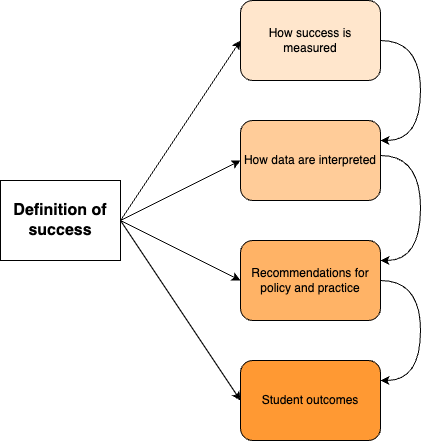
\includegraphics[width=1\linewidth]{res//diagram/sucess-definition-graph.png}
    \caption{Defining success and its impact on the impact\cite{weatherton_success_2021}}
    \label{fig:success_impact}
\end{figure}
From that same research, they approach the importance of correctly defining success within the parameter of the project because defining the goal will inevitably have impact on all part of the research process (as seen in the figure \ref{fig:success_impact}
If we are not able to define success, how can we teach a machine to learn to detect success ? The definition of success will lead to the final measure we are thriving towards. It is certainly one of the trickiest part in this research, and this is why we cannot reach the goal to make a universal machine that would work anywhere anytime, and why we will only provide a framework in order to build similar systems. 

A common recurrent topic on that subject is the lack of holistic approach by academia and researchers on the concept of student success. It is often regarded as a “common sense” where student success is measured not by the score of students, but rather how many got their diplomas. \cite{weatherton_success_2021}.

\paragraph{Conclusion on the human part} is that to create such system, one must fully understand its need and goal with it. You can't train teach a child to count before you know how to count yourself. The question seem simple to answer, if I ask, then I know. But what makes us create such system lies within the same human paradox. Somewhat, what you really need is not what you are seeking for.
\end{document}